\section{Grundlagen des Text Mining}\raggedbottom
Im nachfolgenden Kapitel werden jene Konzepte des \textit{Text Minings} erläutert, welche grundlegend für das Verständnis von Methoden der Textklassifikation sind. Abbildung \ref{pipetk} zeigt die Phasen, die beginnend beim Textkorpus (Sammlung der Ausgangstexte) bis zur abschließenden Einstufung durchlaufen werden. Hieran werde ich mich bei den Ausführungen orientieren.
\begin{figure}[htb]
	\begin{center}
		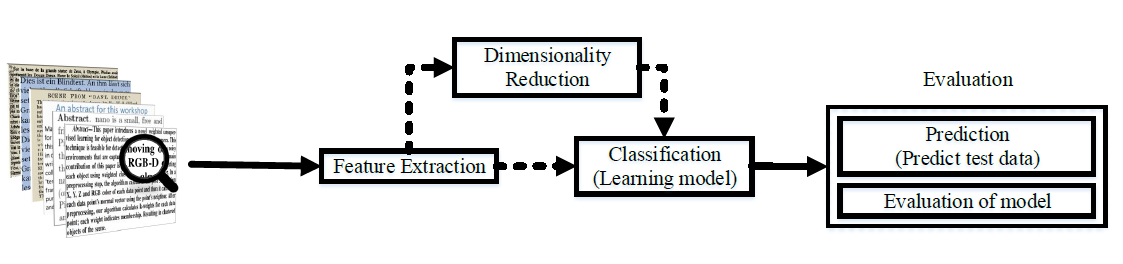
\includegraphics[height=0.25\linewidth, width=0.95\textwidth]{bilder/Abb2v2.png}
		\caption{Pipeline der Textklassifikation \citep{Kow19}  }\label{pipetk}
	\end{center}
\end{figure}
\subsection{Preprocessing}
Der rohe, unbehandelte Text wird beim \textit{Preprocessing} (deutsch: Vorbehandlung) in eine Form überführt, die eine nachfolgende Repräsentation der Daten durch Vektoren und ähnliche Methoden ermöglicht. Je nach gewünschter Anwendung sind hier verschiedene Vorverarbeitungsverfahren in Betracht zu ziehen.\\
Der Begriff Wortsegmentierung bzw. \textbf{Tokenisierung} bezeichnet die Zerteilung des Ausgangstexts in kleinere Einheiten, sogenannte \textit{Token} \citep{MannSch99}. In der Regel handelt es sich hierbei um einzelne Wörter, Zahlen und Satzzeichen. Als grundsätzliches Abgrenzungszeichen gelten in den meisten Sprachen die \textit{Whitespace}-Zeichen (Leerzeichen, Tab, Newline-Zeichen). Dies wird auch auf die zu analysierenden Tweets zutreffen, da diese fast ausschließlich in englischer Sprache verfasst sind.\\
\begin{figure}[htb]
	\begin{center}
		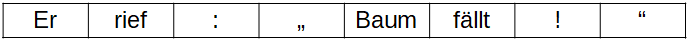
\includegraphics[width=\textwidth]{bilder/tokensatz.png}
		\caption{Tokenisierung eines Beispielsatzes}\label{tokenization}
	\end{center}
\end{figure}\\
Eine weitere Methode der Vorverarbeitung ist das Entfernen von \textbf{Stoppwörtern}. Dies sind sehr häufig auftretende Wörter wie \glqq der\grqq, \glqq die\grqq, \glqq das\grqq, \glqq und\grqq{} oder \glqq von\grqq, welche vornehmlich eine grammatikalische Funktion und keinen Informationsgehalt haben. (vgl. ebd., S. 533)\\
Bei der \textbf{Lemmatisierung} \citep{Air06} werden mehrere Wörter unterschiedlicher Erscheinungsform, welche aber die gleiche Bedeutung haben, auf eine gemeinsame Grundform (genannt Lemma) zurückgeführt.  So lassen sich beispielsweise die deklinierten Substantive \glqq Wortes\grqq, \glqq Wörter\grqq, \glqq Wörtern\grqq auf \glqq Wort\grqq{} zurückführen, während die Grundform der konjugierten Verben \glqq schrieb\grqq, \glqq schreibe\grqq, \glqq schreibst\grqq{} und \glqq schreibt\grqq{} der Infinitiv \glqq schreiben\grqq ist. Ein verwandtes Konzept wird \textbf{Stemming} \citep{Air06} genannt. Der Unterschied zur Lemmatisierung besteht darin, dass das daraus resultierende Grundwort (hier: Stamm) kein natürlichsprachliches Wort sein muss, sondern in der Regel ein um Präfix und Suffix beschnittes Wort ist. Ein Beispiel hierfür ist die Reduzierung der Wörter \glqq gehen\grqq, \glqq umgehen\grqq und \glqq zugehen\grqq{} auf den Stamm \glqq geh-\grqq.\\
Für die Lemmatisierung eines Textes wird auch das \textbf{Part-of-Speech (POS) Tagging} \citep{Kuma15} benötigt. Hierbei wird einem Token seine Wortart (z.B. Nomen, Verb, Adjektiv) oder ein anderes Label wie \glqq Interpunktion\grqq{} zugewiesen. Werkzeuge, die dieses Verfahren anwenden, werden POS-\textit{Tagger} genannt.
\subsection{Feature Extraction}
Bevor eine Klassifikation vorgenommen werden kann, müssen die Merkmale aus den vorliegenden Texten gewonnen und mit mathematischen Methoden strukturiert bzw. modelliert werden. Hierbei fällt die Wahl zumeist auf Vektorisierung.\\
Die einfachste Vektorisierungstechnik ist die \textbf{Bag-of-Words} (BoW) \citep{Ramos13}. Hier wird ein Text durch einen Vektor mit den Begriffshäufigkeiten (auch: \textit{Term Frequencies} (\textbf{TF})) aller zuvor extrahierten Tokens des Textkorpus repräsentiert. Bei einem Beispielkorpus mit den beiden Texten \glqq my coffee is too hot\grqq{} und \glqq my tea is too cold\grqq{} und dem zuvor extrahierten Vokabular
\begin{flushleft}
	\hfil\{ "my", "coffee", "hot", "tea", "cold" \}
\end{flushleft}
ergibt sich die folgende Repräsentation:
\begin{flushleft}
	\hfil$v_1$ = [ 1, 1, 1, 0, 0 ]\\
	\hfil$v_2$ = [ 1, 0, 0, 1, 1 ]
\end{flushleft}
Eine Erweiterung dieser TF-Methode ist \textit{Term Frequency-Inverse Document Frequency} (\textbf{TF-IDF}) \citep{Ramos13}.  Hier wird die Vorkommenshäufigkeit anders gewichtet, um dem Aspekt gerecht zu werden, dass einige Begriffe überproportional oft vorkommen. Gleichung \ref{tfidf_weight} zeigt die Gewichtung 
\begin{equation}
	w(d,t) = TF(d,t) \cdot \log \left( \frac{N}{{DF}(t)} \right)
	\label{tfidf_weight}
\end{equation} 
wobei $N$ die Anzahl der Texte im Korpus und ${DF}(t)$ die Anzahl der Texte, welche den Begriff $t$ enthalten, ist.\\
Eine Möglichkeit, Wortkombinationen bzw. bestimmte Formulierungen als Merkmal zu berücksichtigen ist das \textbf{N-Gramm} \citep{Kow19}. Dies ist die Zusammenfassung von $N$ aufeinanderfolgenden Token in einem Text. Folglich handelt es sich bei den Elementen einer Bag of Words um 1-Gramme. Das nachfolgende Beispiel zeigt die Repräsentation des Textes \glqq Hier sehen Sie ein Beispiel.\grqq{} mit 2-Grammen:
\begin{flushleft}
	\hfil \{ \grqq Hier sehen \grqq, \grqq sehen Sie\grqq, \grqq Sie ein\grqq, \grqq ein Beispiel\grqq \}
\end{flushleft}
Alle vorausgegangenen Methoden der Merkmalsextraktion haben gemeinsam, dass sie keinen Aufschluss über Zusammenhänge der Wortbedeutungen (Semantik) geben. Dieses Problem versuchen die Techniken der \textbf{Worteinbettung} zu lösen. Ein prominentes Beispiel ist \textbf{Word2Vec} \citep{Mikolov13}. Die Grundidee ist hier, dass Begriffe, die eine ähnliche Bedeutung haben, in einem ähnlichen Kontext verwendet werden. Auf dieser Basis wird ein Vektor für jedes Wort im Vokabular durch ein neuronales Netz erzeugt. Die Entfernungen im daraus entstehenden Vektorraum geben dabei semantische Ähnlichkeiten wieder.
\subsection{Dimensionalitätsreduktion}
Bei sehr umfangreichen Datensätzen wie den mehr als 600.000 Tweets in dieser Arbeit werden in der Anwendung der zuvor beschriebenen Verfahren meist hochdimensionale Vektoren erzeugt. In der Folge werden viele Operationen bei späteren Algorithmen der Textklassifikation eine hohe Zeit- und Speicherkomplexität besitzen. Diesem Effekt versucht man im Voraus durch Dimensionalitätsreduktion entgegenzuwirken.\\
Ein erstes verwendetes Verfahren ist die Hauptkomponentenanalyse bzw. \textbf{Principal Component Analysis} (PCA) \citep{Jol02}. Mit diesem ist es möglich, in der Punktwolke der vorhandenen Vektoren all jene Vektor-Komponenten herauszufinden, die für die größte Varianz verantwortlich sind, also den größten Informationsgehalt haben. Der mathematische Mechanismus dahinter ist die Hauptachsentransformation: Es wird eine Ladungsmatrix aus den Eigenvektoren der Kovarianzmatrix gebildet, aus welcher der Anteil der Varianz jeder Komponente an der Gesamtvarianz ersichtlich ist. In der Folge können Komponenten, welche wenig Varianz beitragen, ohne nennenswerten Informationsverlust verworfen werden.\\
Eine andere Möglichkeit ist die \textbf{Nichtnegative Matrixfaktorisierung} (NMF) \citep{LeeSeung99}. Hier wird aus den $n$ Texten mit insgesamt $m$ Wörtern eine $m \times n$ Matrix gebildet, welche approximativ so faktorisiert wird, dass
\begin{center}
	$V \approx W H$
\end{center}
gilt, wobei W eine $m \times r$ Matrix und H eine $r \times n$ Matrix ist. Die $r$ Spalten von $W$ enthalten semantisch verwandte Wörter, welche zusammen einen Kontext bzw. ein Thema bilden. Voraussetzung für dieses Verfahren ist die Nichtnegativität von $V$.\pagebreak